\section{製品目標値を満たすロボットの設計}\label{ux88fdux54c1ux76eeux6a19ux5024ux3092ux6e80ux305fux3059ux30edux30dcux30c3ux30c8ux306eux8a2dux8a08}

基準となるロボット,手先加速を上げるために再設計を行ったロボット,強度を上げるために再設計を行ったロボットの3種類についての解析を踏まえて,当初の製品目標値を満たすアームロボットを設計する.

\subsection{最終のロボットアームの形状}\label{ux6700ux7d42ux306eux30edux30dcux30c3ux30c8ux30a2ux30fcux30e0ux306eux5f62ux72b6}

最終的には,図\ref{last-robot-arm}のような形状のアームを設計した.

\begin{figure}[htbp]
  \begin{center}
    \begin{tabular}{c}
      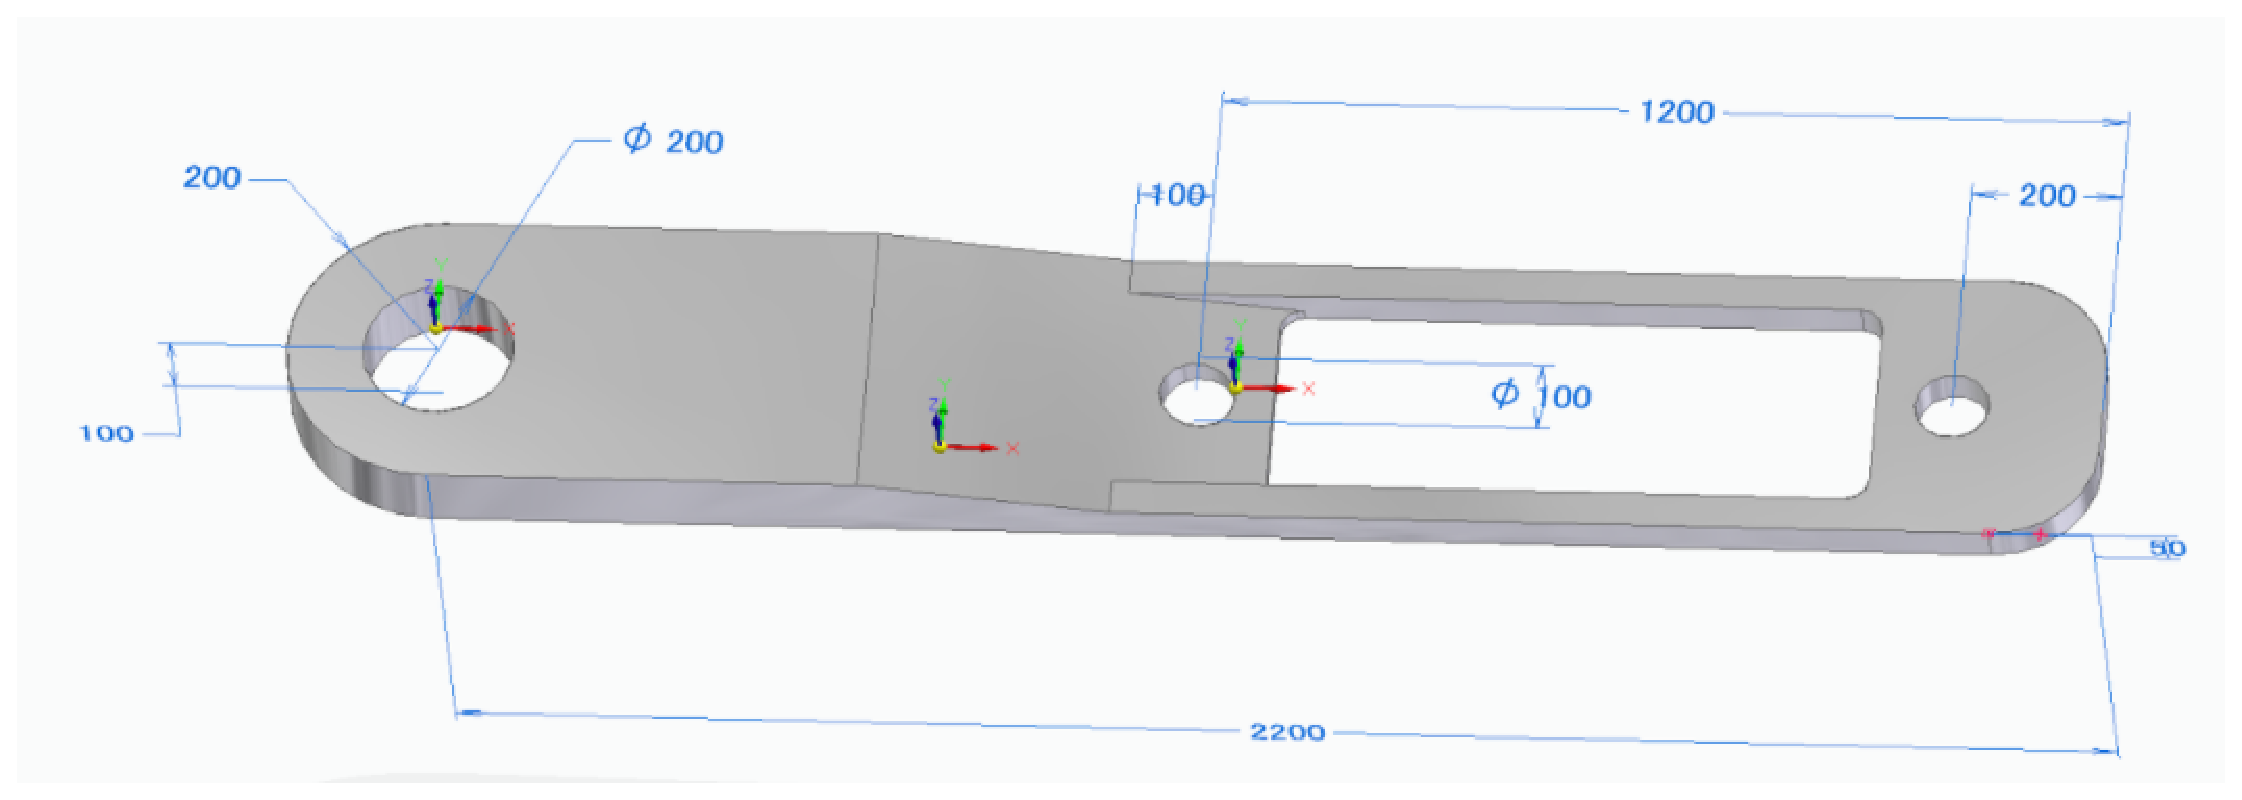
\includegraphics[height=6.0cm]{img/eps/last-robot-arm.eps}
    \end{tabular}
    \caption{アームの最終形状}
    \label{last-robot-arm}
  \end{center}
\end{figure}

根元部分を太くすることで,強度を高めつつ,手先に近い部分をくり抜くことで慣性モーメントを減らし,手先加速度を上げるように設計を行った.また,安全率および許容たわみに余裕があったため,全体的に薄くすることで手先加速度の向上を図った.

\subsection{最終のロボットアームの各種値}\label{ux6700ux7d42ux306eux30edux30dcux30c3ux30c8ux30a2ux30fcux30e0ux306eux5404ux7a2eux5024}

最終的なロボットアームの各種値を表\ref{last-robot-data}に示す.

\begin{table}[htb]
\caption[]{リンクアームの各値}
  \begin{center}
    \begin{tabular}{|c|c|} \hline
      材質 & アルミニウム1060 \\ \hline
      密度 [$\rm kg/m^3$]& 2712.0 \\ \hline
      体積[$\rm m^3$] & 0.0803 \\ \hline
      質量[kg] & 217.781.832 \\ \hline
      慣性モーメント[$\rm kg m^2$] & 223.529  \\ \hline
    \end{tabular}
    \label{last-robot-data}
  \end{center}
\end{table}

アームを全体的に薄くし,質量及び体積を大幅に小さくした.そして手先に近い部分をくり抜くことで慣性モーメントを小さくした.

また,回転中心の軸とアームの重心の軸はSolid
Edgeを使用して計測した結果,0.755{[}m{]}の距離があることがわかった.そこで,軸間距離\(d=0.755[\rm m]\),重心周りの慣性モーメント\(I_G=100.098[\rm kgm^2]\)及び質量\(M=217.781[\rm kg]\)を平行軸の定理に代入すると,式\ref{solvelastKansei}となる.

\begin{eqnarray}
  I &=& I_G+d^2M \nonumber \\
    &=& 100.098 + 0.755^{2} 217.781 \nonumber \\
    &=& 224.239
  \label{solvelastKansei}
\end{eqnarray}

よって,今回の慣性モーメントの値は理論値と一致している事がわかる.

\subsection{最終のロボットアームの応力及び変位}\label{ux6700ux7d42ux306eux30edux30dcux30c3ux30c8ux30a2ux30fcux30e0ux306eux5fdcux529bux53caux3073ux5909ux4f4d}

次に,最終のロボットアームの応力および変位についてシミュレーションし,シミュレーション結果の妥当性をほかのアームロボットの応力及び変位と比較することで確認する.

最終のロボットアームの応力図を図\ref{last-ouryoku}に示す.

\begin{figure}[htbp]
  \begin{center}
    \begin{tabular}{c}
      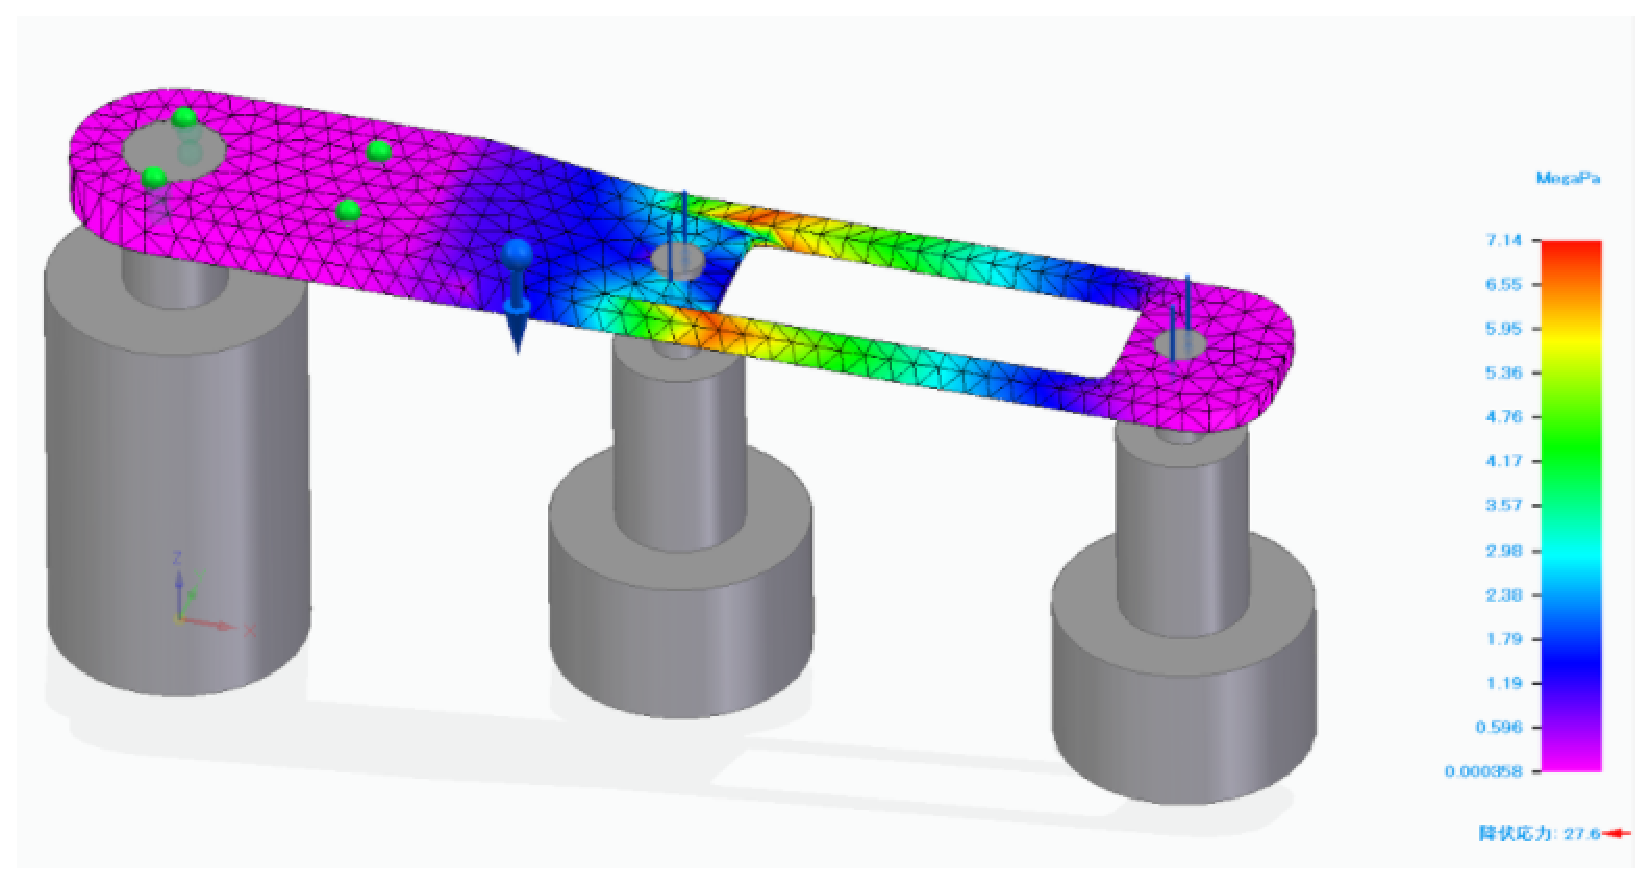
\includegraphics[height=8.0cm]{img/eps/last-ouryoku.eps}
    \end{tabular}
    \caption{最終のロボットアームの応力図}
    \label{last-ouryoku}
  \end{center}
\end{figure}

この時,図\ref{last-ouryoku-result}に示す結果がSolid
Edgeより出力された.

\begin{figure}[htbp]
  \begin{center}
    \begin{tabular}{c}
      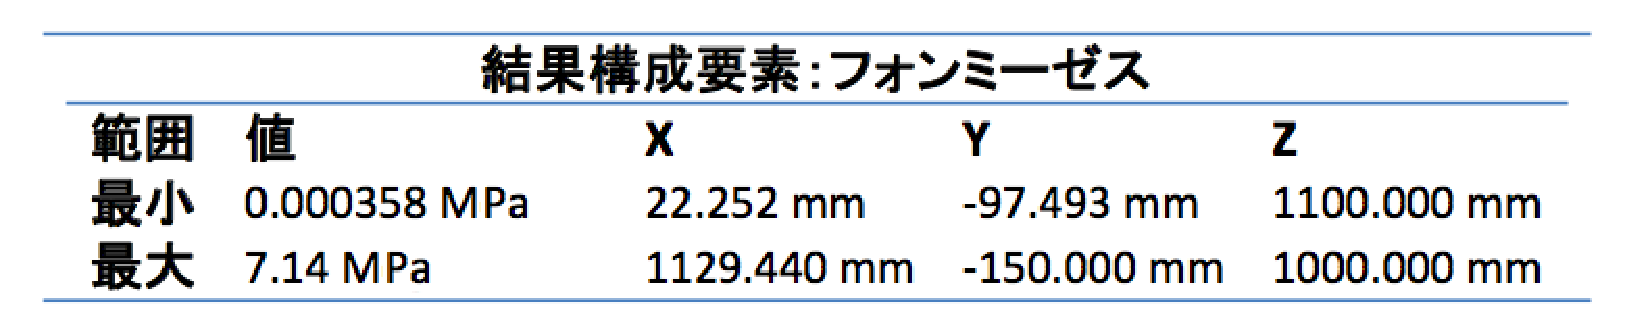
\includegraphics[height=2.7cm]{img/eps/last-ouryoku-result.eps}
    \end{tabular}
    \caption{最終ロボットの応力解析結果}
    \label{last-ouryoku-result}
  \end{center}
\end{figure}

先ほど設計した3種類のアームロボットよりも薄くしたため,理論的には応力は大きくなるはずであり,シミュレーションを行った所,実際に応力は大きくなっているためシミュレーションの内容は正しいことがわかる.

許容応力は27.6{[}MPa{]}であるので,安全率は式\ref{last-anzen}より,3.87となる.

\begin{eqnarray}
  安全率 &=& \frac{許容応力}{最大応力} = 3.87
  \label{last-anzen}
\end{eqnarray}

次に,重力及び荷重によってかかる変位についてシミュレーションし,そのシミュレーション結果の妥当性について検討する.

Solid
Edgeのシミュレーション機能を用いて変位を解析した所,変位分布は図\ref{last-heni}となった.

\begin{figure}[htbp]
  \begin{center}
    \begin{tabular}{c}
      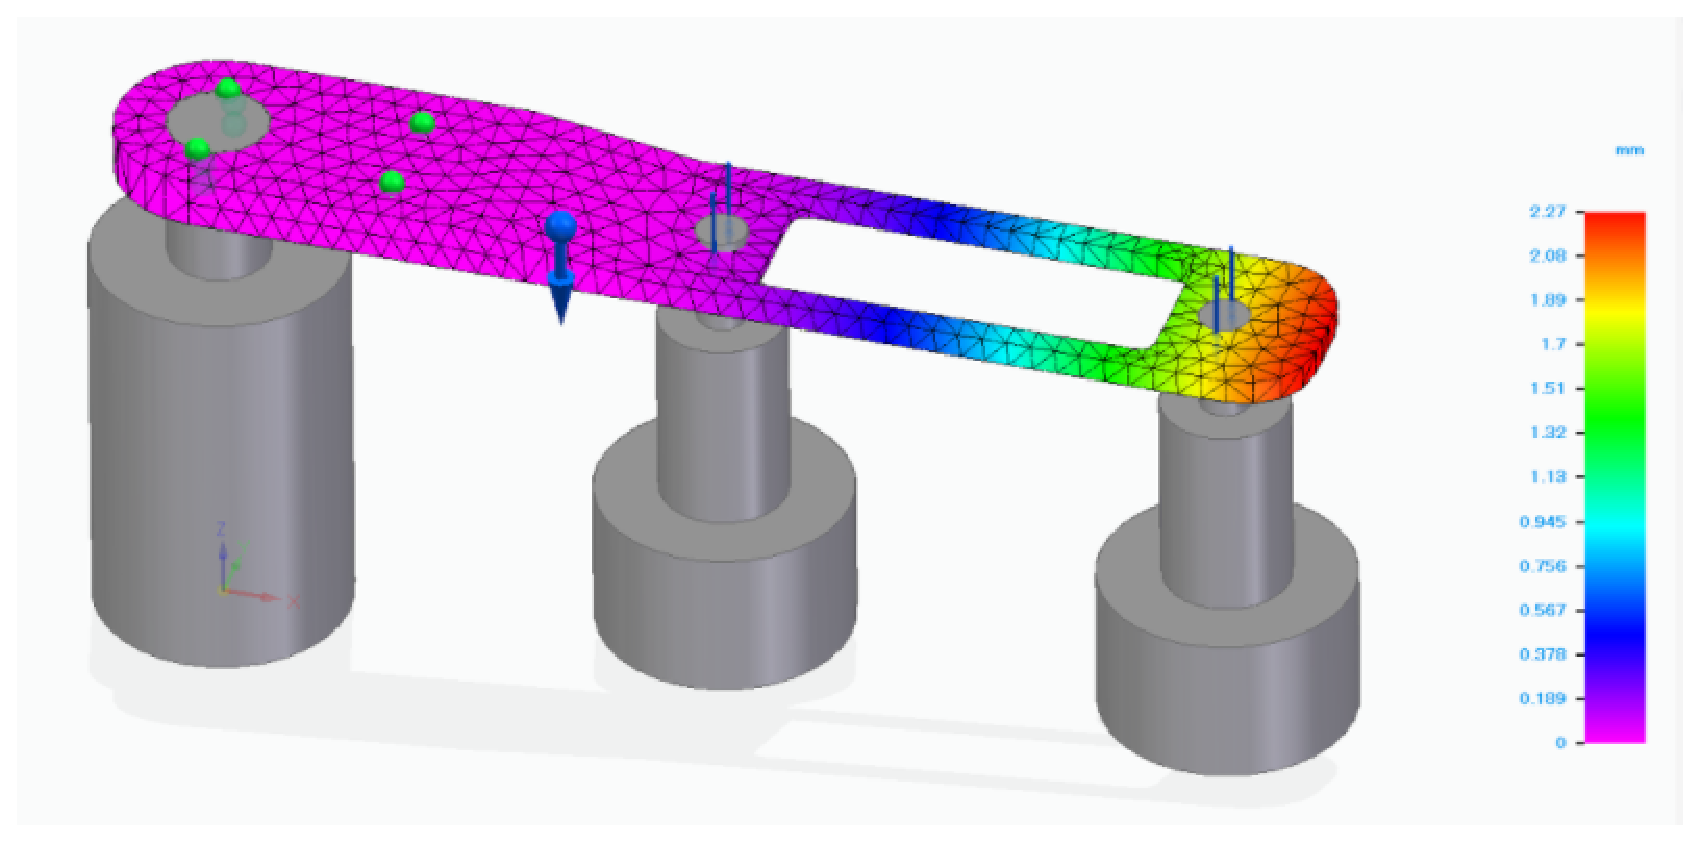
\includegraphics[height=5.7cm]{img/eps/last-heni.eps}
    \end{tabular}
    \caption{最終ロボットの変位分布}
    \label{last-heni}
  \end{center}
\end{figure}

この時,図\ref{last-heni-result}に示す変位結果がSolid
Edgeより出力された.

\begin{figure}[htbp]
  \begin{center}
    \begin{tabular}{c}
      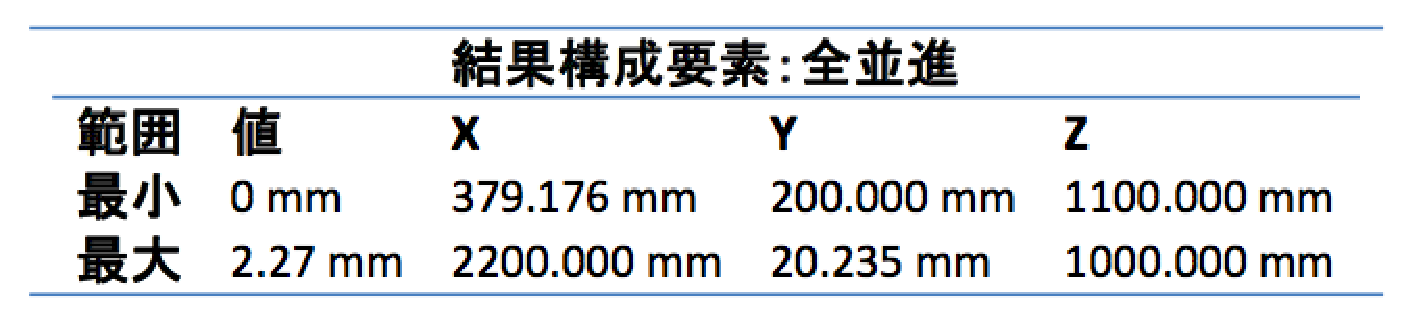
\includegraphics[height=2.5cm]{img/eps/last-heni-result.eps}
    \end{tabular}
    \caption{最終ロボットの変位解析結果}
    \label{last-heni-result}
  \end{center}
\end{figure}

軽量化のために全体的に薄くしたため,変位が先ほど作成した3つのロボットの変位と比較して大きくなっているのは正しい結果といえる.

\subsection{最終ロボットの機構解析について}\label{ux6700ux7d42ux30edux30dcux30c3ux30c8ux306eux6a5fux69cbux89e3ux6790ux306bux3064ux3044ux3066}

SimXpertを使用して,今回作成したアームロボットの関節回転角度を求めた結果を図\ref{last-kaiten}に示す.

\begin{figure}[htbp]
  \begin{center}
    \begin{tabular}{c}
      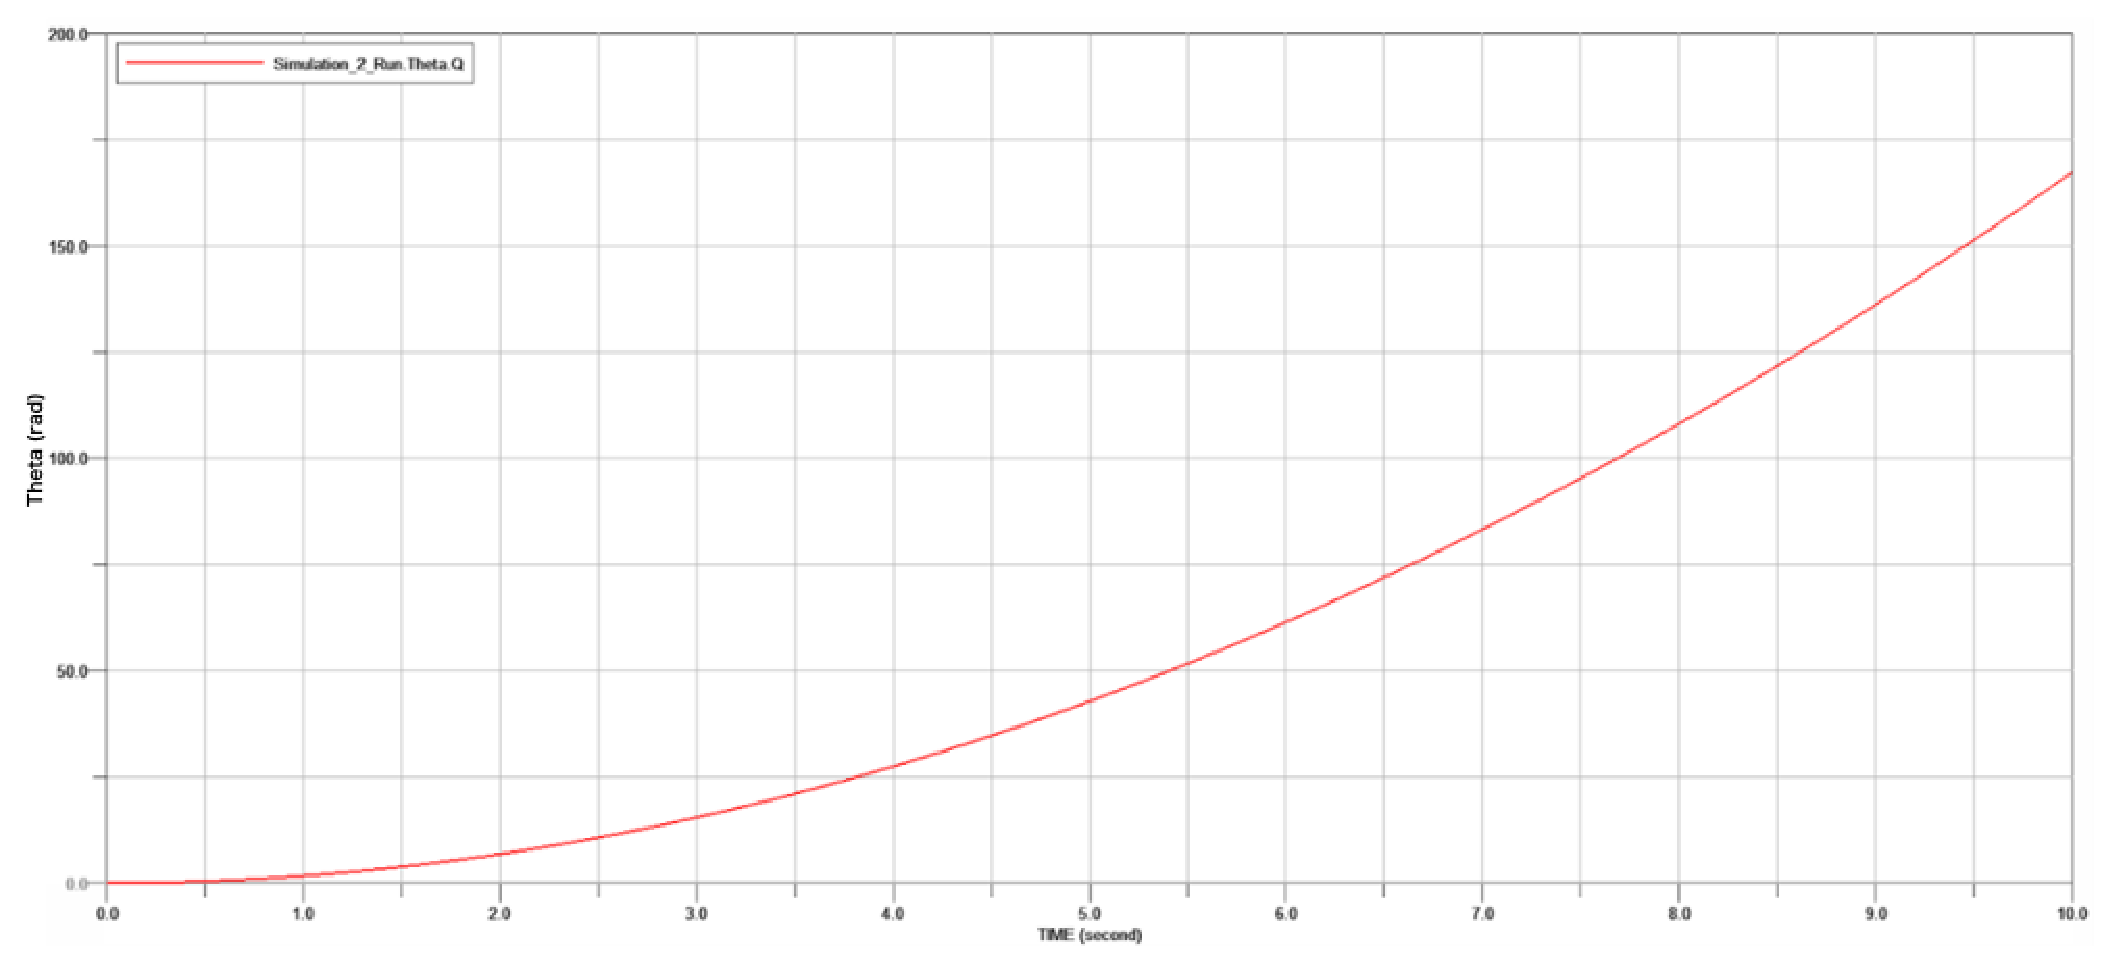
\includegraphics[height=7.5cm]{img/eps/last-kaiten.eps}
    \end{tabular}
    \caption{最終ロボットのアームの関節回転角}
    \label{last-kaiten}
  \end{center}
\end{figure}

SimXpertから得られたこの結果から,最小二乗法を用いて二次の多項式で関節回転角を表すと式\ref{last-deg}となる.

\begin{eqnarray}
  \frac{d\theta}{dt} &=& 1.634t^2+0.484x-0.473 \nonumber \\
  &\approx& 1.634t^2
  \label{last-deg}
\end{eqnarray}

関節角速度\(\frac{d\theta}{dt}\)は式\ref{last-deg}を両辺\(t\)で時間微分することで得られ,式\ref{last-ddeg}となる.

\begin{eqnarray}
  \frac{d\theta}{dt} = 3.268t
  \label{last-ddeg}
\end{eqnarray}

ここで,角速度\(\frac{d\theta}{dt}\)と手先速度の大きさ\(v\)の間には,式\ref{last-hand-vel}の関係がある.ただし,回転中心と手先間の距離を\(r\)と置いた.

\begin{eqnarray}
  v &=& r\frac{d\theta}{dt}
  \label{last-hand-vel}
\end{eqnarray}

式\ref{last-ddeg},及び式\ref{last-hand-vel}より,手先速度の大きさの理論解は式\ref{hand-velocity}となる.

\begin{eqnarray}
  v &=& r(3.268t) \nonumber \\
    &=& 2(3.268t) \nonumber \\
    &=& 6.536t
  \label{hand-velocity}
\end{eqnarray}

ここで,SimXpertを使って得た手先速度の大きさを図\ref{last-tesaki-sokudo}に示す.

\begin{figure}[htbp]
  \begin{center}
    \begin{tabular}{c}
      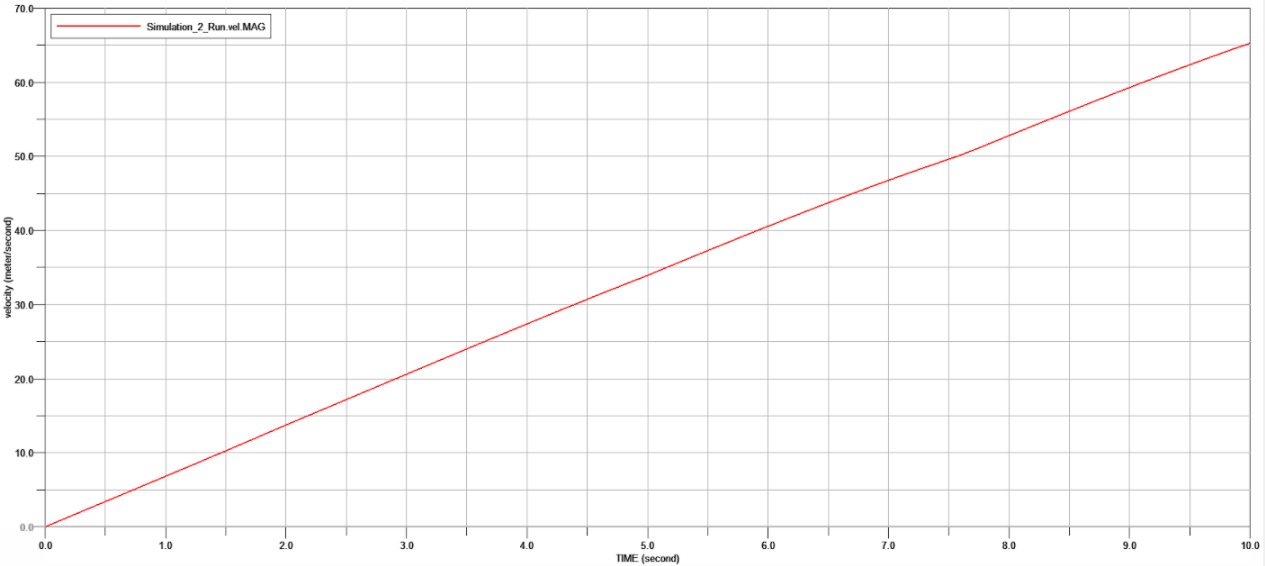
\includegraphics[height=6.5cm]{img/eps/last-tesaki-sokudo.eps}
    \end{tabular}
    \caption{手先速度のシミュレーション結果}
    \label{last-tesaki-sokudo}
  \end{center}
\end{figure}

図\ref{last-tesaki-sokudo}の手先速度\(v\)を最小二乗法を使って一次式で近似すると,式\ref{last-kinji}となる.

\begin{eqnarray}
  v &=&  6.541
  \label{last-kinji}
\end{eqnarray}

手先速度の大きさの理論解と,SimXpertのシミュレーションによって得た手先速度の大きさが一致するので,シミュレーションは正しいといえる.

手先加速度は,手先速度を時間で微分したものなので,6.541{[}\(\rm m/s^2\){]}となる.

\subsection{製品目標値との比較}\label{ux88fdux54c1ux76eeux6a19ux5024ux3068ux306eux6bd4ux8f03}

最終的なロボットの各種値と,最初に決めた製品目標値との比較を行う.

許容最大たわみ,手先加速度,加速時間及び安全率の4つが仕様を満たすようにアームを設計することが今回の目的であったため,この4項目について比較を行う.

表\ref{last-spec}に製品目標値と最終的なロボットの各種値を示す.

\begin{table}[htb]
\caption[]{食品撹拌ロボットの製品目標値・設計仕様}
  \begin{center}
    \begin{tabular}{|c|c|c|c|} \hline
      項目名 & 最終的ロボット & 製品目標値 & 条件\\ \hline \hline
      手先速度[rad/s] & 6.541 & 6.28以上 & 満たす \\ \hline
      加速時間[s] & 1.92 & 2.0以内 & 満たす\\ \hline
      許容最大たわみ(z軸方向) [mm] & 2.27 & 2.50以下 & 満たす\\ \hline
      安全率 & 3.87 & 3.0以上 &満たす\\ \hline
    \end{tabular}
    \label{last-spec}
  \end{center}
\end{table}

以上より,今回設計したロボットは当初設定した製品目標値及び設計仕様を満たしていることが分かる.

\section{おわりに}\label{ux304aux308fux308aux306b}

本課題を通して,以下の知見を得た

\begin{itemize}
\item
  関節駆動トルクを一定のまま高速性の追求には,慣性モーメントを出来る限りする必要があり,慣性モーメントを小さくするには回転軸から遠い場所を軽量化すれば良い.
\item
  必要強度の確保のためには,大きい応力がかかる根本部分を太く設計することによって断面積を大きくし,応力を小さくすれば良い.
\item
  手先加速度にもとづいて設計した後に強度をあげるために再設計を行うと手先加速度が小さくなってしまい何度も再設計をする必要がでてくるため,まずは強度を指標にして設計を行い,そこから強度が落ちないように軽量化及び高速化をしていくと設計がしやすい.
\item
  軽量化の際にアームに穴を開ける際,四角形の穴を開けると穴の角の部分に応力集中が起こり,結果的に応力が大きくなってしまうので穴の形は円形もしくはフィレットをつけるとよい.
\end{itemize}
